\documentclass[12pt]{article}

\usepackage{amsmath}
\usepackage{amssymb}
\usepackage{graphicx}
\usepackage{algpseudocode}
\usepackage[scale=1.0, left=1.25cm, right=1.25cm, top=2.25cm, bottom=1.25cm]{geometry}
\DeclareMathOperator*{\argmin}{arg\,min}

\pagestyle{myheadings}
\markright{CSE 202 Homework 4 \hfill Matthias Springer, A99500782\hfill}

\begin{document}

\section*{Problem 2}
\subsection*{Basic Idea}
\begin{itemize}
	\item $\mathit{PERFECT\-ASSEMBLY} \in \mathcal{NP}$: a permutation $P$ of $s_i \in S$ is a certificate that can be checked in polynomial time by ensuring that $\bigcup P = S$, and $|P| = |S|$, and for every consequtive pair $p_i$, $p_{i+1}$ in $P$, $p_i[l+1, 2l] \circ p_{i+1}[1, l] \in T$\footnote{$\circ$ is string concatenation and $\mathit{str}[a,b]$ denotes the substring from index $a$ to $b$ (inclusive) of $\mathit{str}$.}.
	\item $\mathit{PERFECT\-ASSEMBLY}$ is $\mathcal{NP}$-hard: $\mathit{HAMILTONIAN\-PATH} \leq_P \mathit{PERFECT\-ASSEMBLY}$
	\begin{itemize}
		\item For every $v \in V$, generate a string $vv$ in $S$.
		\item For every $(u,v) \in E$, generate a string $uv$ in $T$.
		\item $G=(V,E)$ has a hamiltonian path iff $S$ has a perfect assembly with respect to $T$.
	\end{itemize}
\end{itemize}

\subsection*{Proof: $\mathit{PERFECT\-ASSEMBLY} \in \mathcal{NP}$}
\begin{itemize}
	\item A certificate $\mathit{str}$ is a string permutation of all $s_i \in S$, such that every consequtive pair $(s_i, s_{i+1})$ is corroborated by a string in $T$.
	\item First, we check if $\mathit{str}$ is in fact a permutation of $S$ by checking if all consequtive substrings of lengths $2l$ are elements of $S$, if there are duplicates among these substrings, and ensure that the number of the substrings equals $|S|$. This can be done in polynomial time by comparing every such substring in $\mathit{str}$ with each other (find duplicates) and finding every such string in $S$.
	\item Then, we check if every consequtive pair of substrings of length $2l$ in $\mathit{str}$ is corraborated by a string $t_k \in T$. This is the case if, for two substrings $s_i$, $s_{i+1}$, $s_i[l+1, 2l] \circ s_{i+1}[1, l] \in T$.
\end{itemize}

\subsection*{Proof: $\mathit{PERFECT\-ASSEMBLY}$ is $\mathcal{NP}$-hard}
We show that $\mathit{HAMILTONIAN\-PATH} \leq_P \mathit{PERFECT\-ASSEMBLY}$. We know that $\mathit{HAMILTONIAN\-PATH}$ is $\mathcal{NP}$-hard. We show how to generate an instance of $\mathit{PERFECT\-ASSEMBLY}$ and show that it has a solution if and only if there exists a hamiltonian path.

\subsubsection*{Generate instance of $\mathit{PERFECT\-ASSEMBLY}$}
Given an instance of $\mathit{HAMILTONIAN\-PATH}$ with $G=(V,E)$, we generate an instance of $\mathit{PERFECT\-} \\ \mathit{ASSEMBLY}$ as follows.

\begin{itemize}
	\item $\Sigma = V$, where $\Sigma$ is the alphabet.
	\item $S = \{vv \left.\right| v \in V\}$
	\item $T = \{uv \left.\right| (u,v) \in E\}$
	\item $l = 1$
\end{itemize}

\subsubsection*{$\mathit{HAMILTONIAN\-PATH} \Rightarrow \mathit{PERFECT\-ASSEMBLY}$}
\begin{itemize}
	\item Let $G=(V,E)$ be a graph that contains a hamiltonian path with $|V| = n$.
	\item Then there is a sequence $(i_1, i_2, \ldots i_n)$, such that $(v_{i_1}, v_{i_2}, \ldots,  v_{i_n})$ is a hamiltonian path.
	\item Then $\mathit{str} = v_{i_1}v_{i_1}v_{i_2}v_{i_2} \ldots v_{i_n}v_{i_n}$ is a certificate that proves that $S = \{v_{i_1}v_{i_1}, v_{i_2}v_{i_2}, \ldots, v_{i_n}v_{i_n}\}$ is a perfect assembly with respect to $T$, because $\mathit{str}$ is a permutation of $S$ (therefore, we visit every vertex exactly once) and, for every consequtive pair $v_iv_iv_{i+1}v_{i+1}$, there must be an edge $(v_i,v_{i+1}) \in E$ (otherwise, this would not be a path in $G$ at all).
\end{itemize}

\subsubsection*{$\mathit{PERFECT\-ASSEMBLY} \Rightarrow \mathit{HAMILTONIAN\-PATH}$}
\begin{itemize}
	\item Let $G=(V,E)$ be a graph with $|V|=n$ and let $S$ be a perfect assembly with respect to $T$.
	\item Then, there must be a certificate $\mathit{str}$ such that $\mathit{str}$ is a permutation of $S$. Therefore, for $\mathit{str} = v_{i_1}v_{i_1}v_{i_2}v_{i_2} \ldots v_{i_n}v_{i_n}$, $P=(v_{i_1}, v_{i_2}, \ldots, v_{i_n})$ is a permutation of $V$.
	\item $P$ is a hamiltonian path because it visits every vertex exactly once and, for every consequtive pair of vertices $(v_{k}, v_{k+1})$, there exists an edge $(v_k, v_{k+1}) \in E$, because every consequtive pair in $\mathit{str}$ is corroborated by a $t_j \in T$, and all $t_j \in T$ represent edges in $G$ by definition.
\end{itemize}

\subsubsection*{Complexity of Reduction}
$|\Sigma| = |S| = |V|$, $|T| = |E| = \mathcal{O}(|V|^2)$, $l = 1$, and $|s_i| = 2$ for every $s_i \in S$. Therefore, all quantities of the generated instance are polynomial in the number of vertices $|V|$ and the instance can be generated in polynomial time.

\section*{Problem 5}
\subsection*{Subproblem a: Solve in $\mathcal{O}(2^n \cdot p(n))$ time}

\subsubsection*{Basic Idea}
\begin{itemize}
	\item Solve with dynamic programming: Let $\mathit{HAM}[S, s, t]$ be true iff there is a hamiltonian $s$-$t$ path in $S \subseteq V$.
	\item $\mathit{HAM}[S, s, t] = \bigvee_{k \in S} \mathit{HAM}[S - \{t\}, s, k] \wedge (k, t) \in E$
	\item Intuition: There is a hamiltonian path from $s$ to $t$ in $S$, if there is a hamiltonian path from $s$ to some $k \in S$ in $S-\{t\}$ and $(k,t) \in E$.
\end{itemize}

\subsubsection*{Dynamic Programming Table}
\begin{itemize}
	\item Base case for subsets of size one: $\forall a_1 \in V, a_2 \in V, a_3 \in V: \mathit{HAM}[\{a_1\}, a_2, a_3] := a_1 = a_2 = a_3$
	\item $\forall s \in V, t \in V, S \subseteq V, |S| > 1: \mathit{HAM}[S, s, t] = \bigvee_{k \in S} \mathit{HAM}[S - \{t\}, s, k] \wedge (k, t) \in E$
	\item We fill the table with increasing cardinalities of $S$, i.e. we first fill the table for all subsets $S$ with $|S|=2$, then for all subsets $S$ with $|S|=3$, and so on. Notice, that, in the recursive definition, we only use table entries with a subset $S$ that has a smaller cardinality.
\end{itemize}

\subsubsection*{Full Algorithm}
\begin{itemize}
	\item Fill the dynamic programming table for all base cases.
	\item Fill the dynamic programming table according to the recursive definition as described in the previous section.
	\item Check all values $\mathit{HAM}[V, a, b]$ for all $a \in V, b \in V$. If at least one of them is true, then there is a hamiltonian path in the graph.
\end{itemize}

\subsubsection*{Space Complexity}
The size of the table is $2^{|V|} \cdot |V| \cdot |V|$, so the space complexity is exponential in the number of vertices.

\subsubsection*{Runtime Complexity}
\begin{itemize}
	\item Filling the dynamic programming base cases: $|V|^3$ entries.
	\item Filling the rest of the table according to the recursive definition: there are $\mathcal{O}(2^{|V|} \cdot |V|^2)$ table entries and for every entry we iterate over all $k \in S$, where $|S| \leq |V|$. Therefore, this takes $\mathcal{O}(2^{|V|} \cdot |V|^3) = \mathcal{O}(2^{|V|} \cdot p(|V|))$ time.
	\item We scan the table for all $a \in V, b \in B$ at $\mathit{HAM}[S, a, b]$. This takes $\mathcal{O}(|V|^2)$ time.
	\item The overall runtime complexity is $\mathcal{O}(2^{|V|} \cdot |V|^3)$. 
\end{itemize}

\subsubsection*{Proof}
We prove by induction over the size of $|S|$ that algorithm is correct.

\begin{itemize}
	\item \emph{Induction Base:} Let $S \subseteq V$ with $|S| = 1$. Then, there can be hamiltonian $s$-$t$ path if and only if $s=t$ and $S=\{s\}$, because we only take a look at the subgraph with this single vertex. Therefore, $\mathit{HAM}[\{a\}, s, t] := a = s = t$.
	\item \emph{Induction Hypothesis:} Let $\mathit{HAM}[S, s, t] = \mathit{true}$ if and only if there is a hamiltonian $s$-$t$ path in $S \subseteq V$, for all $|S| \leq k$.
	\item \emph{Induction Proof:} We want to decide whether there is a hamiltonian $s$-$t$ path in $S \subseteq V$ with $|S|=k+1$. A hamiltonian path is a sequence of vetices $(v_1, v_2, \ldots, v_{k+1})$. Such a hamiltonian path exists if and only if a hamiltonian path $(v_1, v_2, \ldots, v_k)$ exists in $S - \{v_{k+1}\}$ and there is an edge $(v_k, v_{k+1}) \in E$ in $G$. Therefore, $\mathit{HAM}[S, s, t] = \bigvee_{k \in S} \mathit{HAM}[S - \{t\}, s, k] \wedge (k, t) \in E$ for $|S| > 1$. From the induction hypothesis, we know the correct value of $\mathit{HAM}[T, a, b]$ for $a \in V, b \in V, T \subseteq V, |T| = k$.
	\item A hamiltonian path can start and end at any vertex. Therefore, there is a hamiltonian path in $G$, iff $\mathit{HAM}[V, a, b] = \mathit{true}$ for at least one combination of $a \in V, b \in V$.
\end{itemize}

\subsection*{Subproblem b: Solve in polynomial space}
\subsubsection*{Basic Idea}
\begin{itemize}
	\item The basic idea relies on the concept of alternate addition/substraction from the lecture.
	\item We count the number of all paths (starting at $v_1$ and ending at $v_n$) of size $|V|$ (that use $|V| - 1$ edges) in $G=(V,E)$.
	\item A path of length $|V|$ is not hamiltonian iff at least one vertex $v$ was not visited. Therefore, for every $v \in V$, we substract the number of paths of length $|V|$ in $G'=(V-\{v\}, E')$, i.e. all paths that do not visit $v$.
	\item Notice, that we substracted paths that miss two vertices twice. We can make up for this by adding all pathes of size $|V|$ that miss two vertices. But now we added paths that miss three vertices too often. We keep adding and substracting in such a way.
	\item Counting all these pathes takes exponential time because we eventually have to examine all subsets $S \subseteq V$ for paths of size $|V|$. Notice, that we do not need a DP table here, resulting in polynomial space complexity.
	\item We repeat this process for all possible start and end vertices.
\end{itemize}

\subsubsection*{Full Algorithm}
We run the following algorithm for every pair $s \in V, t \in V$ and return $\mathit{true}$ if at least one run returns $\mathit{true}$.

\begin{algorithmic}
	\State $\mathit{counter} \gets 0$
	\State $\mathit{sign} \gets 1$

	\For{$k \gets |V| \mbox{ \textbf{downto} } 1$}
		\ForAll{$S \subseteq V \wedge |S| = k$}
			\State $\mathit{counter} \gets \mathit{counter} + \mathit{sign} \cdot \mathit{countPaths}((S, E'), s, t)$
		\EndFor

		\State $\mathit{sign} \gets -\mathit{sign}$
	\EndFor
	
	\Return $\mathit{true} \mbox{ \textbf{iff} } \mathit{counter} > 0$
\end{algorithmic}

The function $\mathit{countPaths}((V, E), s, t)$ counts the number of all paths of length $|V|$ in $(V, E)$ that start at $s$ and end at $t$. This can be done with a modified version of BFS. Note, that it is allowed to visit vertices and edges multiple times.

\subsubsection*{Proof}
\begin{itemize}
	\item $\mathit{countPaths}((V,E), s, t)$ counts the number of $s$-$t$ paths of size $|V| - 1$ in $G=(V,E)$.
	\item Let $\mbox{missing}[i]$ be the number of $s$-$t$ paths in all graphs with $i$ vertices missing from $V$. E.g. $\mathit{missing}[1]$ is the number of $s$-$t$ paths in all graphs $G=(V', E')$ with $V'=V-\{v\}$ for every $v \in V$.
	\item A graph $G=(V,E)$ contains a hamiltonian path if there is at least one $s$-$t$ path for some $s \in V, t \in V$ where no vertex is missing in the path. We can determine the number of these paths by substracting the number of paths in all graphs with one vertex missing from the number of paths in the graph with no vertex missing. The number of these paths is $\mathit{missing}[0] - \mathit{missing}[1] + \mathit{missing}[2] - \mathit{missing}[3] + \ldots$. We have to use this alternating sum because we counted the number of paths with two vertices missing in the graphs multiple times in $\mathit{missing}[2]$. Then, again, we counted some paths multiple times, yielding this alternating sum.
\end{itemize}

\subsubsection*{Finding all $s$-$t$ paths of length $|V| - 1$}
\begin{itemize}
	\item We maintain an array $\mbox{counter}[v_i, d]$ that counts how often we encounter the vertex $v_i$ with a current distance of $d$.
	\item At the beginning, $\mbox{counter}[s,0] = 1$ and all other array slots are initialized to $0$.
	\item We run BFS and maintain tuples of \emph{vertex} $v$ and \emph{current distance} $d$ in the queue.
	\item For every tuple $(v,d)$, we traverse all outgoing edges $(v,u) \in E$ and increase the counter for $u$ at distance $d+1$ by the counter for the current tuple $\mbox{counter}[v, d]$.
	\item Note, that BFS traverses tuples $(v, d)$ with increasing values of $d$, i.e. before a tuple $(v, d')$ with $d'> d$ is processed, all tuples $(u, d)$ have been processed. Therefore, we will never increase the counter for an already processed tuple.
	\item $\mathit{counter}[t, |V| - 1]$ contains the number of $s$-$t$ paths of length $|V| - 1$.
\end{itemize}

\begin{algorithmic}
	\State $\mathit{counter}[v_i, d] \gets 0 \mbox{   } \forall v_i \in V, 0 \leq d \leq |V|$
	\State $\mathit{counter}[s, 0] \gets 1$
	\State $Q \gets \mbox{ new Queue}$
	\State $Q.\mbox{add}((s, 0))$
	\While{$|Q| > 0$}
		\State $p=(v, d) \gets Q.\mbox{pop}()$
		\ForAll{$(e=(v, u) \in E$}
			\If{$d+1 < |V| \wedge (u, d+1) \not\in Q$}
				\State $Q.\mbox{push}((u, d+1))$
			\EndIf

			\State $\mbox{counter}[u, d+1] \gets \mbox{counter}[u, d+1] + \mbox{counter}[v, d]$
		\EndFor
	\EndWhile

	\Return $\mathit{counter}[t, |V|-1]$
\end{algorithmic}

This algorithm fills $|V| \cdot (|V| - 1) = \mathcal{O}(|V|^2)$ array slots, and for every array slot $(v,d)$, the algorithm traverses all of $v$'s incident nodes $u$ with $(v,u) \in E$. Therefore, the runtime complexity for this algorithm is $\mathcal{O}(|V|^2 \cdot |E|) = \mathcal{O}(|V|^4)$. The space complexity is $\mathcal{O}(|V|^2)$, i.e. the size of the array.

\subsubsection*{Runtime Complexity}
\begin{itemize}
	\item Generating all subsets $S \subseteq V$ in the for loop: $\mathcal{O}(2^{|V|})$ total iterations.
	\item One run of $\mathit{countPaths}$ per subset: $\mathcal{O}(2^{|V|} \cdot |V|^4)$.
	\item Running the whole algorithm for all pairs of $s \in V, t \in V$: $\mathcal{O}(2^{|V|} \cdot |V|^6)$.
\end{itemize}

\subsubsection*{Space Complexity}
\begin{itemize}
	\item The space for the current subset $S$ and the $\mathit{counter}$ variable and the $\mathit{sign}$ variable is constant.
	\item Every run of $\mathit{countPaths}$ requires $\mathcal{O}(|V|^2)$ temporary space, i.e. this space is only required during one run of the function.
	\item The overall space complexity of the algorithm is $\mathcal{O}(|V|^2)$.
\end{itemize}

\section*{Problem 3}
\subsection*{Basic Idea}
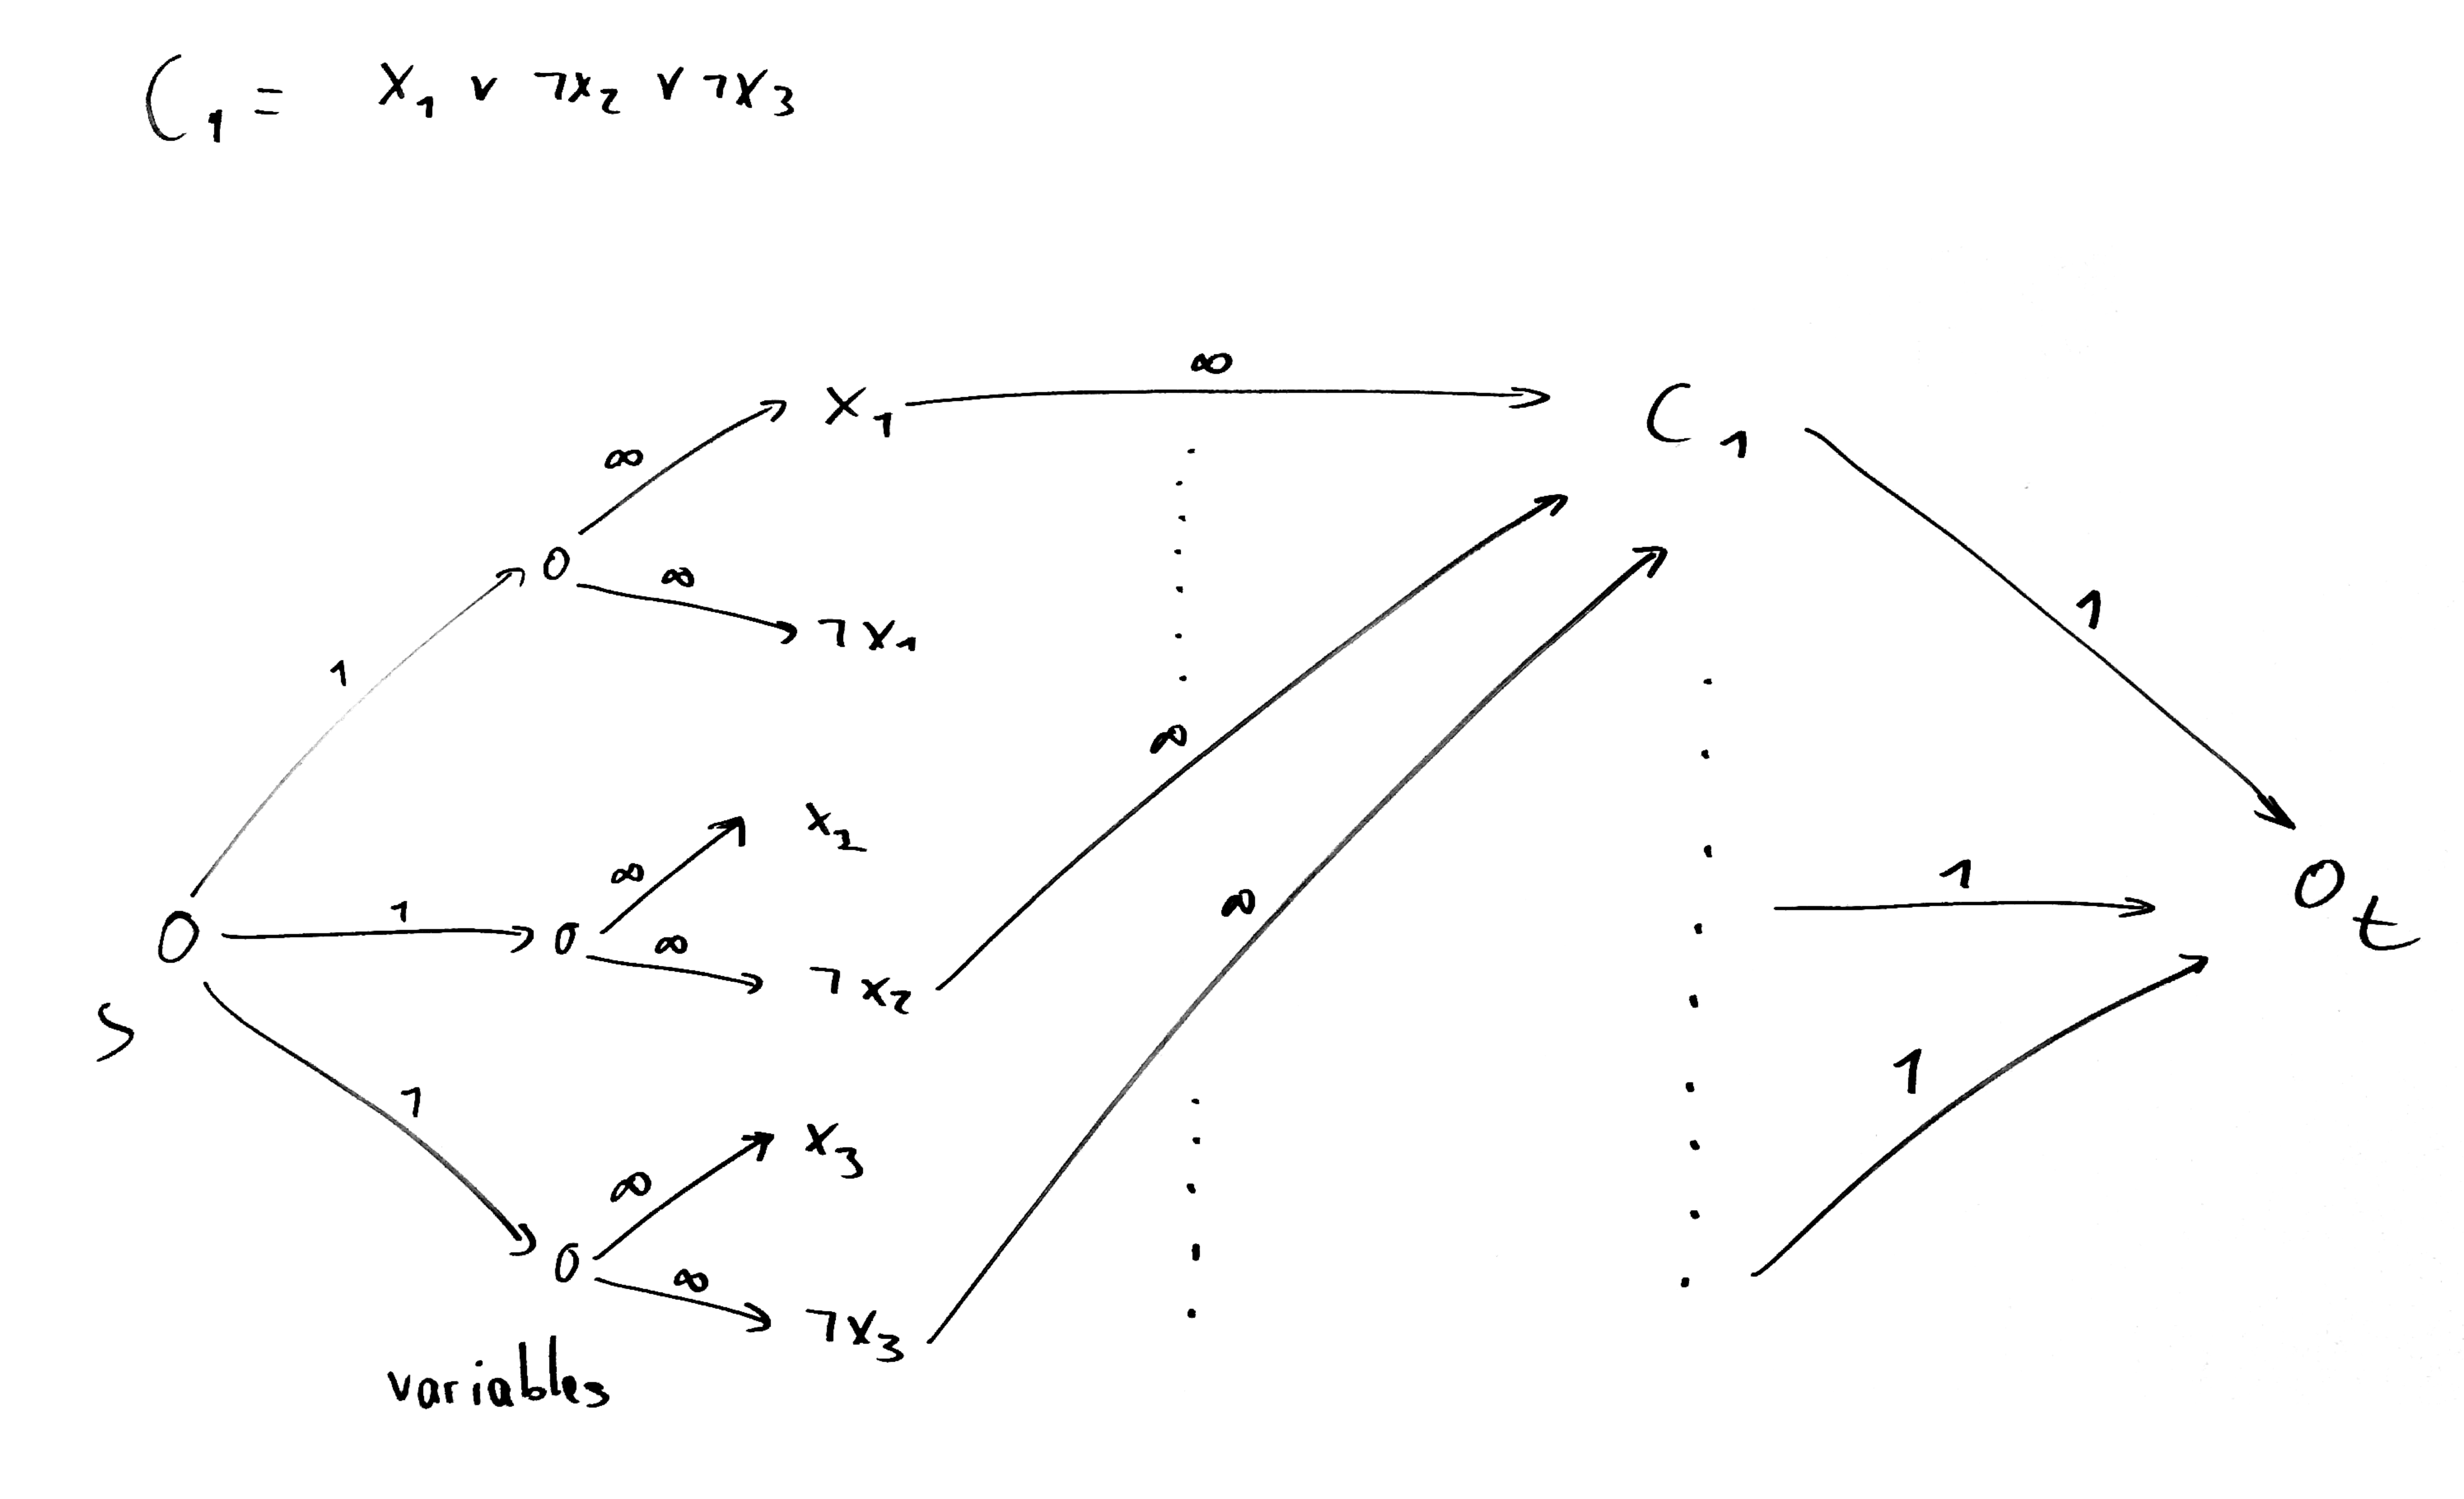
\includegraphics[width=\textwidth]{3_1.pdf}
\begin{itemize}
	\item The number of clauses must be equal to number of variables, because every variable must appear in exactly 3 clauses.
	\item We build a flow network as illustrated above. Every variable can send a flow of $1$ to its positive or negative literal and every literal can satisfy clauses it appears in. We only allow it to satisfy one clause. In fact, a literal could sometimes satisfy more than one clause, but we can always find an assignment such that every variable satisfies exactly one clause\footnote{According to Hall's theorem. See proof for details.}. The capacity constraints on the edges leading to the sink $t$ ensure that every clauses uses only one literal for satisfiability.
	\item There is a valid assignment of variables iff the max flow value is $n$. A variable is set to $\mathit{true}$ if its positive literal receives a flow of $1$. Otherwise, it is $\mathit{false}$.
\end{itemize}

\subsection*{Flow Network Construction}
\begin{itemize}
	\item Add a source $s$ and a sink $t$.
	\item For every variable $x_i$, add a node $v_{x_i}$ and two literal nodes $l_{x_i}$ and $l_{\neg x_i}$.
	\item Add edges $(s, v_{x_i})$ with a capacity of $1$, and edges $(v_{x_i}, l_{x_i})$ and $(v_{x_i}, l_{\neg x_i})$ with capcities of $\infty$.
	\item For every clause $C_i$, add a node $v_{C_i}$.
	\item Add edges $(v_{C_i}, t)$ with a capacity of $1$.
	\item If $a$ is a literal and $a \in C_i$, add an edge $(l_a, v_{C_i})$ with a capacity of $\infty$.
\end{itemize}

\subsection*{Algorithm}
\begin{itemize}
	\item Build the flow network for the problem instance.
	\item Run the Ford-Fulkerson algorithm to obtain a max flow.
	\item If a literal node $l_{x_i}$ receives a flow of $1$, set $x_i$ to $\mathit{true}$, otherwise set it to $\mathit{false}$.
\end{itemize}

\subsection*{Proof}
\begin{itemize}
	\item \emph{Integrality constraint:} All flow capacities are integers. Therefore, the Ford-Fulkerson algorithm generates an integer flow.
	\item \emph{Valid assignment:} All variable nodes can send a flow of either $0$ or $1$ to one of the literals (due to integrality). In case the max flow value is $|\mathit{Variables}|$, i.e. there is a perfect matching\footnote{We show below that this is always the case.}, every variable sends a flow of $1$ to either its positive or negative literal. Therefore, the assignment is valid in a sense that every variable has an assignment and there is no contradiction.
	\item \emph{Perfect matching}
	\begin{itemize}
		\item  According to Hall's theorem, a bipartite graph $G=((\mathit{Variables}, \mathit{Clauses}), E)$ has a matching of size $\mathit{Variables}$, if and only if, for every $S \subseteq \mathit{Variables}$, $|N(S)| \geq |S|$, where $N(S)$ is the set of vertices in $\mathit{Clauses}$ that are reachable from $S$.
		\item In the graph, we have additional nodes for positive and negative literals for every variable. When we think about a matching, we consider the variable nodes to be directly connected to the clause nodes. This is does not change anything in the following argument.
		\item Let $S \subseteq \mathit{Variables}$. $N(S) \geq \max \{3, |S|\}$, because every variable appears in exacly 3 clauses. Therefore, 3 is a lower bound for $S \not= \emptyset$. For $|S|$ variables, we have $3|S|$ literals appearing in some clauses. Since every clause has exaclty 3 literals, we need at least $\frac{3|S|}{3} = |S|$ clauses. Therefore, $S$ is connected to at least $|S|$ clauses.
	\item Therefore, there is always a matching of size $\mathit{Variables}$, i.e. there is always a perfect matching. Therefore, this version of $\mathit{3\-SAT}$ is always satisfiable.
	\end{itemize}
\end{itemize}

\subsection*{Runtime Complexity}
\begin{itemize}
	\item Building the flow network: We create $\mathcal{O}(n)$ nodes for variables/literals and $\mathcal{O}(n)$ nodes for clauses, since the number of clauses equals the number of variables. We add no more than $\mathcal{O}(n^2)$ edges.
	\item The max flow can be calculated with the Edmonds-Karp algorithm in $\mathcal{O}(|V| |E|^2) = \mathcal{O}(n^5)$.
	\item The overall runtime is $\mathcal{O}(n^5)$. Therefore, the runtime complexity is polynomial in the number of variables.
\end{itemize}

\section*{Problem 1}
\subsection*{Basic Idea}
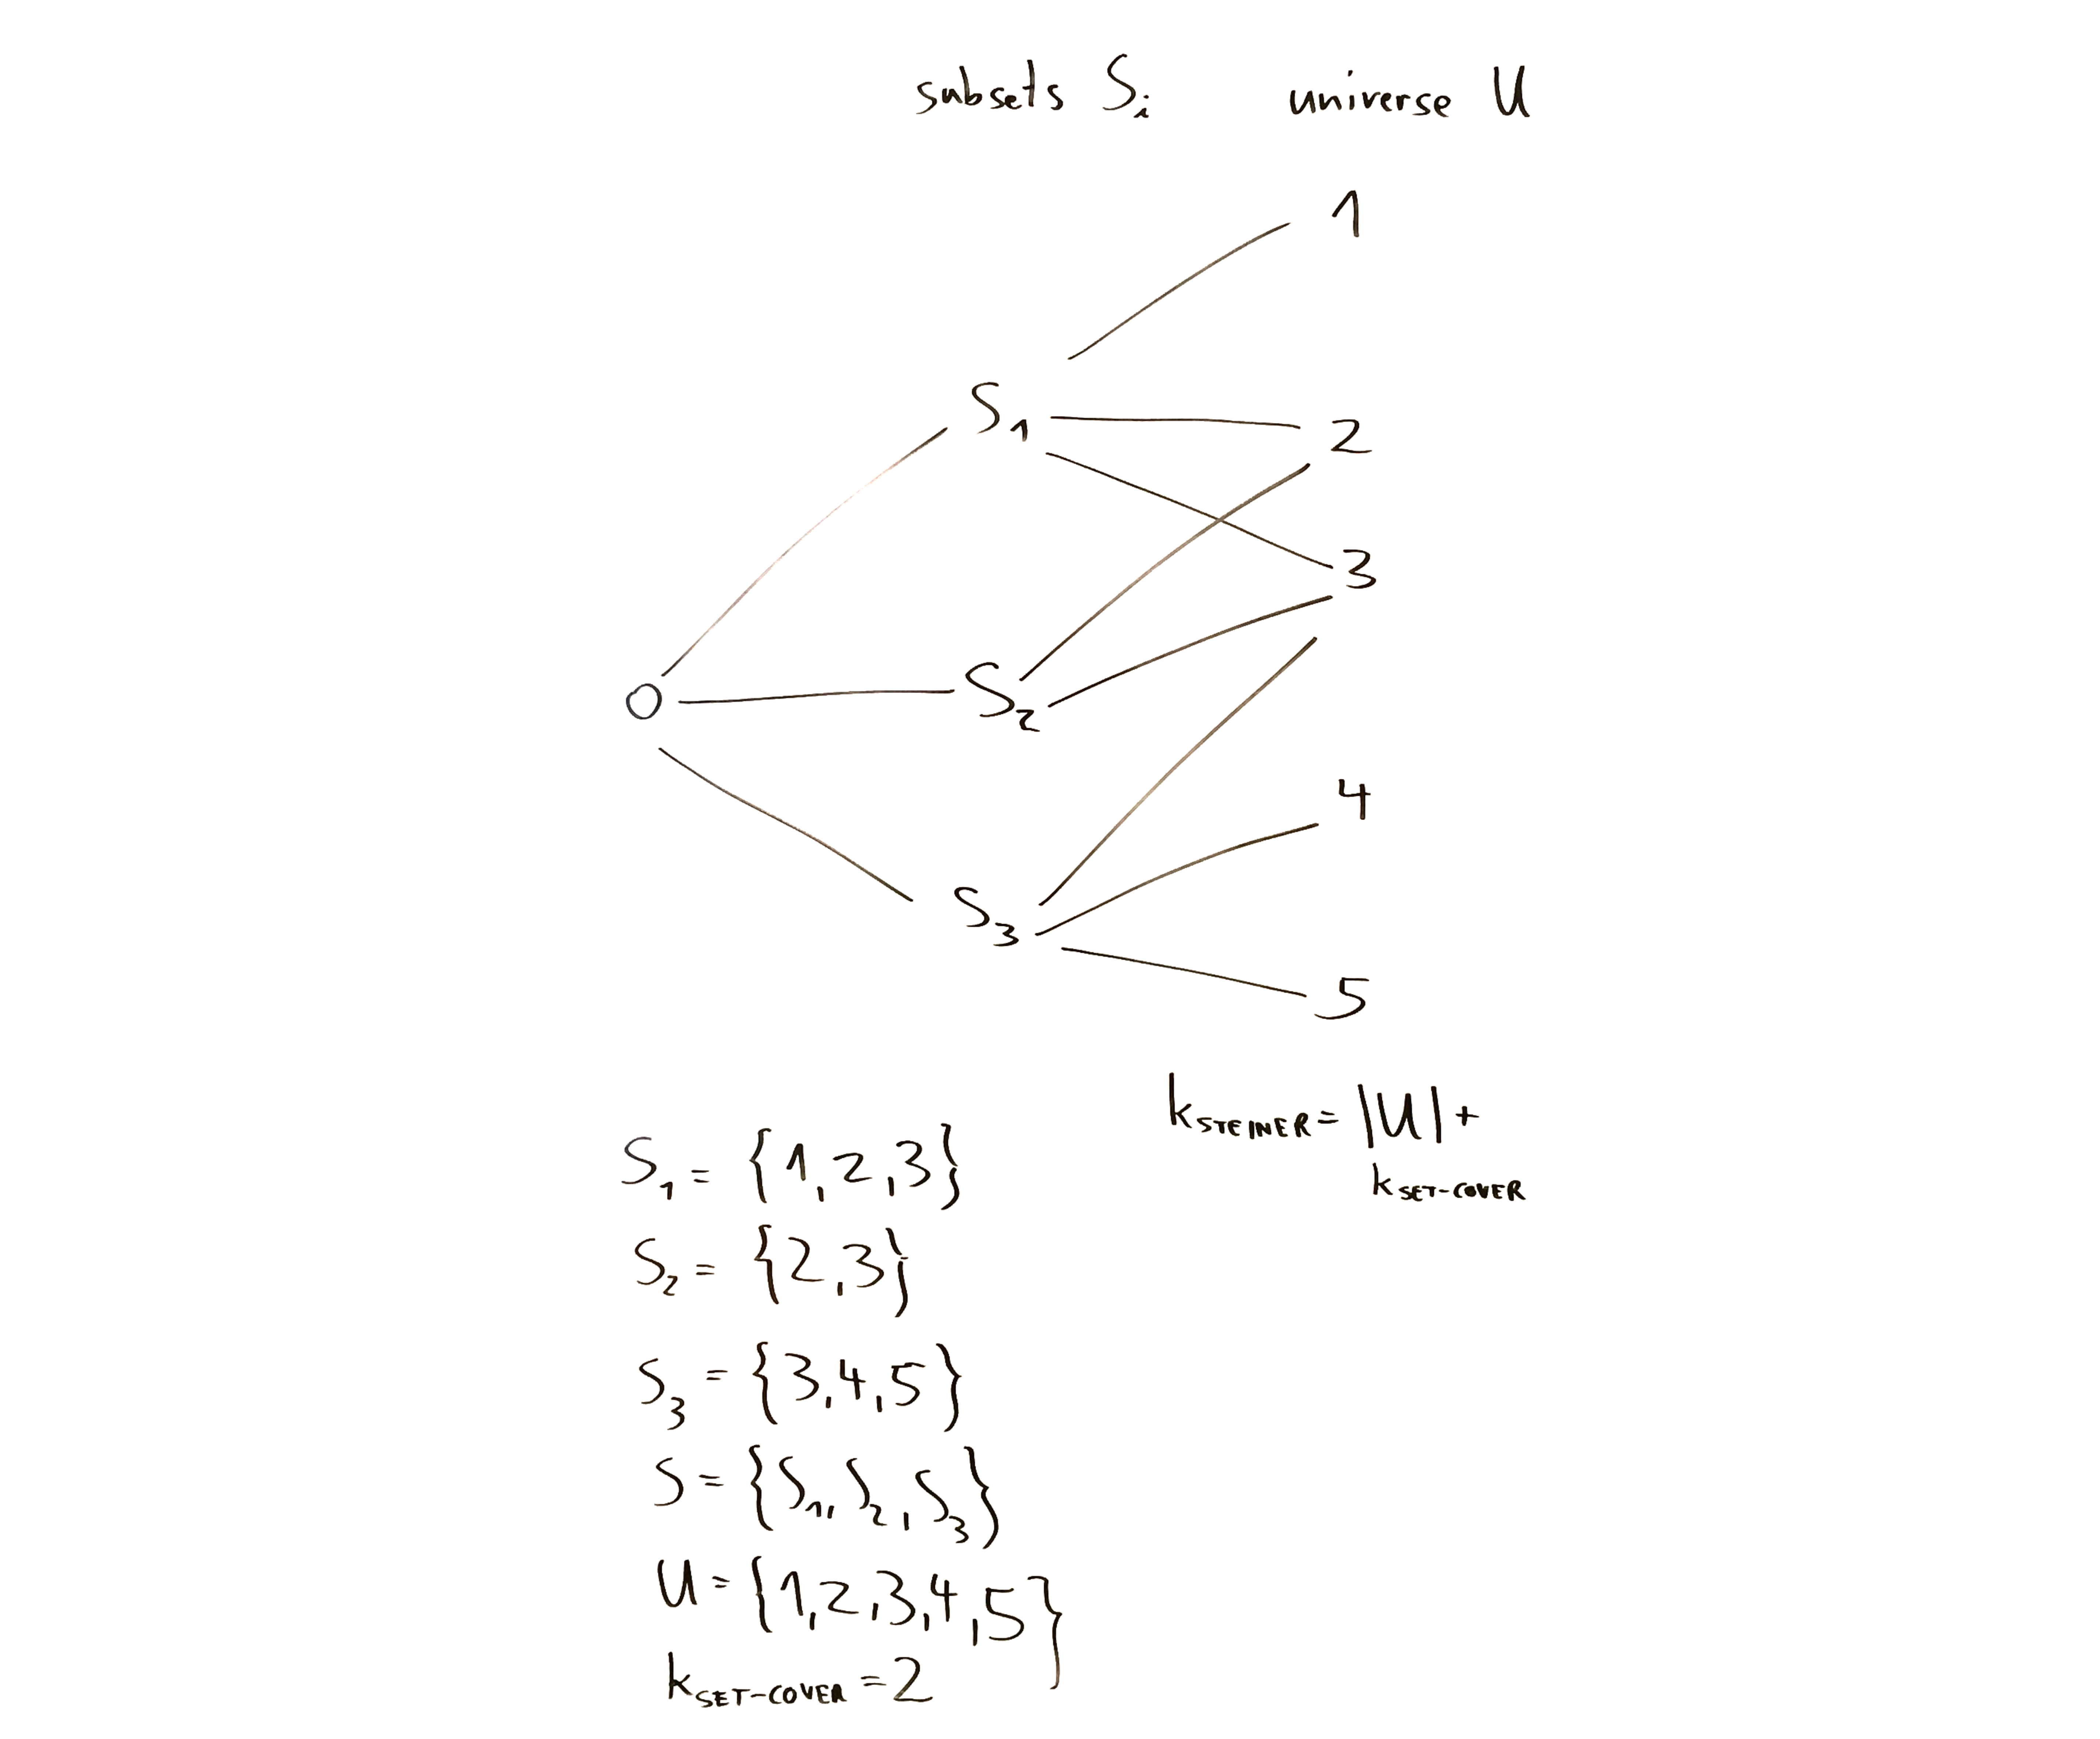
\includegraphics[width=\textwidth]{1_1.pdf}
\begin{itemize}
	\item $\mathit{STEINER} \in \mathcal{NP}$: a subset $F \subseteq E$ of edges is a certificate that can be checked in polynomial time by ensuring that $|F| \leq k$ and that, for an arbitrary edge $(u,v) \in F$, all nodes in $V$ can be reached from $u$. This can be done with DFS.
	\item $\mathit{STEINER}$ is $\mathcal{NP}$-hard: $\mathit{SET\-COVER} \leq_P \mathit{STEINER}$
	\begin{itemize}
		\item For every element $u \in U$ and every subset $S_i \in S$ , generate a vertex.
		\item Connect all subset vertices to a common root vertex and all elements to the subsets they are included in.
		\item $k_{\mathit{STEINER}} = k_{\mathit{SET\-COVER}} + |U|$
		\item There is a set cover of at most $k_{\mathit{SET\-COVER}}$ subsets iff there is a Graphical Steiner Tree with at most $k_{\mathit{STEINER}}$ edges.
	\end{itemize}
\end{itemize}

\subsection*{Proof: $\mathit{STEINER} \in \mathcal{NP}$}
\begin{itemize}
	\item A certificate is a subset $F \subseteq E$.
	\item First, we check if $|F| \leq k$.
	\item Then, we check if the graph induced by $F$ is contains all vertices and is connected. We take an arbitrary edge $(u,v) \in F$ and start a DFS on $u$. There is a Graphical Steiner Tree of at most size $k$ iff the DFS visits all $v \in V$. The DFS can maintain an array of already visited nodes and determine whether all vertices were visited. DFS takes $\mathcal{O}(|V| + |F|) = \mathcal{O}(|V| + |E|)$ time.
\end{itemize}

\subsection*{Proof: $\mathit{STEINER}$ is $\mathcal{NP}$-hard}
We know that $\mathit{SET\-COVER}$ is $\mathcal{NP}$-hard and show how to reduce it $\mathit{STEINER}$.

\subsubsection*{Graph Construction}
We show how to generate a graph for the Graphical Steiner Tree problem from an instance of $\mathit{SET\-COVER}$. Let $I = (U, S, k)$ be an instance of $\mathit{SET\-COVER}$.

\begin{itemize}
	\item Add a root vertex $v_r$.
	\item For every element $u_i \in U$, add a vertex $v_{u_i}$.
	\item For every subset $S_i \in S$, add a vertex $v_{S_i}$.
	\item If $u_i \in S_i$, add an edge $\{v_{u_i}, v_{S_i}\}$.
	\item For every subset $S_i$, add an edge $\{v_r, v_{S_i}\}$.
\end{itemize}

\subsubsection*{Generate instance of $\mathit{STEINER}$}
\begin{itemize}
	\item Build the graph according to the previous section.
	\item Set $k_\mathit{STEINER} = k_\mathit{SET\-COVER} + |U|$.
\end{itemize}

\subsubsection*{$\mathit{SET\-COVER} \Rightarrow \mathit{STEINER}$}
\begin{itemize}
	\item Let $I=(U, S, k)$ be an instance of $\mathit{SET\-COVER}$ that has a set cover $C=\{S_{a_1}, S_{a_2}, \ldots, S_{a_k}\}$ of size $k$.
	\item Then, the according Graphical Steiner Tree graph has the following Steiner Tree with $k+|U|$ edges: select all edges $\{v_r, S_{a_i}\}$ for all $1 
\leq i \leq k$ ($k$ edges). In adddition, select $|U|$ edges $\{S_{a_i}, u\}$ such that all $u \in U$ are covered. There must always be such edges, because $C$ is a set cover, i.e. all $u \in U$ are contained in some sets $S_{a_i} \in C$.
\end{itemize}

\subsubsection*{$\mathit{STEINER} \Rightarrow \mathit{SET\-COVER}$}
\begin{itemize}
	\item Let $I = (U, S, k)$ be an instance of $\mathit{SET\-COVER}$ and $F \subseteq E$ be a set of edges in the Graphical Steiner Tree graph with $|F| \leq k + |U|$.
	\item Then, all vertices $v_{u_i}$ are connected to $v_r$ in $F$. Since there are no connections among the vertices $v_{u_i}$, they must all be connected through some vertices $v_{S_i}$. There cannot be more than $k$ edges $\{v_r, v_{S_i}\}$ in use, because there are $|U|$ edges needed for all $v_{u_i}$ and we have at most $k + |U|$ edegs in $F$. $\{S_i \left.\right| \{v_r, v_{S_i}\} \in F\}$ is a set cover of size $k$, because, according to the graph construction, there is an edge between a vertex $v_{u_i}$ and a subset vertex $v_{S_i}$ if and only if $u_i \in S_i$. Therefore, $\bigcup_{S_i \in S: \{v_r, v_{S_i}\} \in F} S_i = U$.
\end{itemize}

\subsubsection*{Complexity of Reduction}
We generate $\mathcal{O}(|U| + |S|)$ nodes and no more than $\mathcal{O}((|U| + |S|)^2)$ edges. Therefore, the reduction is polynomial in the size of the $\mathit{SET\-COVER}$ instance.

\section*{Problem 4}
\subsection*{Basic Idea}
\begin{itemize}
	\item Dynamic programming: $\mathit{CUT}[T, d]$ is the maximum achievable cut value of subtree $T$, where the difference between the partition set sizes is exactly $d$.
	\item $P = \{T, T_1, T_2\}$, where $T_1$ is $T$'s left child and $T_2$ is $T$'s right child\footnote{As stated in the problem description, we only have binary trees.}.
	\item $\mathit{CUT}[T, d] = \max_{S \subseteq P} \{ \sum_{(a,b) \in S \times P-S} w_{a,b} + \max_{-n \leq a_1, a_2 \leq n \wedge a_1 + a_2 = d - ||P-S| - |S||)} \{ \mathit{CUT}[T_1, a_1] + \mathit{CUT}[T_2, a_2] \} \}$
	\item For all leaves $L_i \in V$: $\mathit{CUT}[L_i,1] = 0$ and for $d \not= 1: \mathit{CUT}[L_i, d] = -\infty$.
	\item For every subtree $T$, it does not matter in which partition set $T$ is. By swapping all nodes in set $A$ and set $B$, $\mathit{CUT}$ stays the same. Therefore, $\forall T \in V, d \in \mathbb{Z}: \mathit{CUT}[T, d] = \mathit{CUT}[T, -d]$.
	\item For every tree, we decide which nodes $P$ are in the same partition set. This decision contributes to the partition size difference with a value of $||P| - |S||$, i.e. the difference of the number of nodes of $P$ in $A$ and in $B$. We must accumulate a difference in partition sizes in the child nodes $T_1$ and $T_2$ of $d-||P| - |S||$, i.e. the difference in partition sizes in $T_1$ and $T_2$ can be arbitrary as long as the total difference in partition size is exactly $d$.
\end{itemize}

\subsection*{Full Algorithm}
\begin{itemize}
\item The following code describes the function $\mathit{calculateCut}(T)$ that fills the dynamic programming table for all nodes in subtree $T$. This function fills the table in a DFS style. It calculates the values for both children first and then calculates the value according to the formula.

\begin{algorithmic}
	\If{$T_1 = \emptyset \wedge T_2 = \emptyset$}
		\State $\mathit{CUT}[T, 1] \gets 0$
		\State $\mathit{CUT}[T, d] \gets -\infty \forall d \in \mathbb{Z}\{1\}: -|V| \leq d \leq |V|$
	\Else
		\If{$T_1 \not= \emptyset$}
			\State $\mathit{calculateCut}(T_1)$
		\Else
			\State $T_1 \gets T_\emptyset$
		\EndIf
		\If{$T_2 \not= \emptyset$}
			\State $\mathit{calculateCut}(T_2)$
		\Else
			\State $T_2 \gets T_\emptyset$
		\EndIf

		\ForAll{$d \in \mathbb{Z}: -|V| \leq d \leq |V|$}
		\State $\mathit{CUT}[T, d] \gets -\infty$
		\ForAll{$S \subseteq \{T, T_1, T_2\}$}
			\State $r \gets \sum_{(a,b) \in S \times (\{T, T_1, T_2\} - S)} w_{a,b}$
			\ForAll{$a_1, a_2 \in \mathbb{Z}: -|V| \leq a_1, a_2 \leq |V| \wedge d = a_1 + a_2 + ||\{T, T_1, T_2\} - S| - |S||$}
				\State $v \gets \mathit{CUT}[T_1, a_1] + \mathit{CUT}[T_2, a_2] + r$
				\If{$v > \mathit{CUT}[T, d]$}
					\State $\mathit{CUT}[T, d] \gets v$
					\State $\mathit{SOL}[T, d] \gets (S, (T_1, a_1), (T_2, a_2))$
				\EndIf
			\EndFor
		\EndFor
		\EndFor
	\EndIf
\end{algorithmic}

\item Then, we invoke the algorithm as follows ($R$ is the root of the tree).

\begin{algorithmic}
	\State $\mathit{CUT}[T_\emptyset, 0] \gets 0$
	\State $\mathit{CUT}[T_\emptyset, d] \gets -\infty \mbox{  } \forall d \in \mathbb{Z}: -|V| \leq d \leq |V|$
	\State $\mathit{calculateCut}(R)$
	\State $\mathit{output}(R \in A)$
	\State $\mathit{printSol}(R, 0, A)$
\end{algorithmic}

\item This function $\mathit{printSol}(T, d, \mathit{side})$ prints the rest of the solution. It retrieves the path of decisions that was made during the actual algorithm from the $\mathit{SOL}$ table.

\begin{algorithmic}
	\State $s \gets \mathit{SOL}[T, d]$
	\State $S \gets s[1]$
	\State $T_1 \gets s[2][1]$
	\State $a_1 \gets s[2][2]$
	\State $T_2 \gets s[3][1]$
	\State $a_2 \gets s[3][2]$
	\ForAll{$(T_c, a_c) \in \{(T_1, a_1), (T_2, a_2)\}$}
	\If{$T_c \not= T_\emptyset$} 
		\If{$T_s \in S = T \in S$}
			\State $\mathit{output}(T_c \in \mathit{side})$
			\State $\mathit{printTable}(T_c, a_c, \mathit{side})$
		\Else
			\State $\mathit{otherSide} \gets A \mbox{ \textbf{if} } \mathit{side} = B \mbox{ \textbf{else} } B$
			\State $\mathit{output}(T_c \in \mathit{otherSide})$
			\State $\mathit{printTable}(T_c, a_c, \mathit{otherSide})$
		\EndIf
	\EndIf
	\EndFor
\end{algorithmic}
\end{itemize}

\subsection*{Proof}
\begin{itemize}
	\item \emph{Independent subproblems:} For two trees $T_1$ and $T_2$, where $T_1$ and $T_2$ are not subtrees of each other, an optimal solution for $T_1$ is independent from an optimal solution for $T_2$, since there are no edges between $T_1$ and $T_2$.
	\item \emph{Optimal substructure:} Given an optimal solution for all child nodes, the algorithm finds an optimal solution for the whole subtree. We prove this by induction.
	\begin{itemize}
		\item \emph{Induction Base:} If $T$ is a leaf, i.e. it has no child nodes, then there are no edges involved at all. Therefore, the cut value is always $0$ and the difference between the sizes of the partition sets must be $1$, i.e. $d=1$, because we only have one vertex that must be in one set. For other values of $d$, the problem is infeasible. We denote this by a cut value of $-\infty$, i.e. the algorithm will never choose it unless the whole problem instance is infeasible.
		\item \emph{Induction Hypothesis:} Assume that for a vertex $T$, we know the optimal solution for all $-|V| \leq d \leq |V|$ for both the left and the right child vertex $T_1$ and $T_2$.
		\item \emph{Induction Proof:} We find the optimal solution for a given value of $d$ by evaluting all possible solutions: we have to decide in which set we put $T$, $T_1$ and $T_2$\footnote{In the algorithm, we consider all possibilities to put these vertices in the set $S$ or not. Actually, this is not necessary, since the symmetric cases, where we switch the partition sets, have the same cut value and partition set size difference. But it doesn't hurt, either.} and think about the subtrees. In fact, it is not important, in what exact set we put the vertices, since we are only interested in the difference of size of the partition sets. To achieve a value of $d$, the difference in the left subtree plus the difference (of partition set sizes) in the right subtree plus the difference of the vertices $T$, $T_1$ and $T_2$ must equal $d$\footnote{Note, that it does not matter whether $T_1$ and/or $T_2$ put more vertices in set $A$ or in set $B$, since both cases are completely symmetric. We can always swap both sets.}. By evaluating all these possibilities, we can be sure to find the optimal solution. We only have to consider values $-|V| \leq d \leq |V|$, the difference of partition size sets cannot be greater than the number of vertices in total\footnote{In fact, for most cases we will have a value of $-\infty$ in the DP table for the lower vertices.}.
	\end{itemize}
\end{itemize}

\subsection*{Runtime Complexity}
\begin{itemize}
	\item We fill the DP table bottom up using DFS. Therefore, we visit each vertex and edge once: $\mathcal{O}(|V| + |E|)$.
	\item For every vertex, we examine all values of $-|V| \leq d \leq |V|$: $\mathcal{O}(|V|)$. For every value of $d$, we examine all possibilities of taking subsets $S$ of $\{T, T_1, T_2\}$: constant. For every subset $S$, we consider all possibilites to achieve a value of $d - ||P-S| - |S||$: $\mathcal{O}(|V|^2)$ possibilities of assigning $a_1$ and $a_2$. In total, we consider $\mathcal{O}(|V|^3)$ cases per vertex.
	\item For every case, we check two values in the DP table (constant time). The runtime complexity for filling the whole table is $\mathcal{O}(|V|^4)$.
	\item Printing the solution is done by visiting every vertex once with a DFS and examining one DP table entry per vertex. The overall runtime complexity for the algorithm is $\mathcal{O}(|E| + |V|^4) = \mathcal{O}(|V|^4)$.
\end{itemize}

\section*{Problem 6}
\subsection*{Subproblem a: Approximation Algorithm}
\subsubsection*{Basic Idea}
\begin{itemize}
	\item Sort all visitors $V_i$ by their value $v_i$ in a decreasing way.
	\item Greedy algorithm: Allocate the next visitor $V_i$ to the the ad $A_j$ that has currently the lowest sum.
\end{itemize}

\subsubsection*{Full Algorithm}
\begin{algorithmic}
	\State $\mathit{sort} \mbox{ $V$ by value}$
	\ForAll{$V_i \in V$}
		\State $\mathit{minAd} \gets \min_{1 \leq i \leq m} A_i$
		\State $\mathit{add} \mbox{ $V_i$ to } \mathit{minAd}$
	\EndFor
\end{algorithmic}

\subsubsection*{Proof of Approximation Factor}
\begin{itemize}
	\item We assume that $n \geq m$. Otherwise, at least one ad does not get any visitor. In that case, the maximum spread is zero for both the optimal algorithm and the greedy algorithm.
	\item Let $T_\mathit{OPT}$ be the maximum spread that is generated by the optimal algorithm. $T_\mathit{OPT} \leq \frac{\sum_{i=1}^n v_i}{m}$, because in case all visitors are equally distributed, the minimum value sum is maximum.
	\item Let $T_G$ be the spread that is generated by the greedy algorithm. Let $A_l$ be the ad with the lowest sum. We denote the sum of the ad $A_i$ with $v_{A_i}$.
	\begin{itemize}
		\item $A_l$ has the lowest sum: $\forall 1 \leq i \leq m: v_{A_l} \leq v_{A_i}$.
		\item Let $L_k$ be the last visitor allocated to $A_k$. $\forall 1 \leq i \leq m: v_{A_l} \geq v_{A_i} - v_{L_i}$. Otherwise, we would have allocated $L_i$ to $A_l$.
		\item In the formula above $v_{A_i} \geq \frac{\sum_{i=1}^n v_i}{m}$, because if this ad was below average, we would have selected $A_l$ instead. $v_{L_i} \leq \frac{\sum_{k=1}^n v_k}{2m}$ according to the problem description.
		\item Therefore, $T_G \geq \frac{\sum_{i=1}^n v_i}{m} - \frac{\sum_{i=1}^n v_i}{2m} = \frac{\sum_{i=1}^n v_i}{2m}$.
	\end{itemize}
	\item Therefore, $T_G \geq \frac{T_\mathit{OPT}}{2}$.
\end{itemize}

\subsection*{Subproblem b}
\begin{itemize}
	\item $m=2$
	\item Visitor values: \{10, 8, 5, 4, 3\}
	\item Optimal solution: $15$ ($A_1 = \{10, 5\}$, $A_2= \{4,8,3\}$)
	\item Greedy algorithm output: $14$ ($A_1 = \{10, 4\}$, $A_2 = \{8,5,4\}$)
\end{itemize}

\section*{Problem 7}
\subsection*{Subproblem a}
\begin{itemize}
	\item Let $T$ be an arbitrary independent set in $G$ and $S$ be an independent set generated by the greedy algorithm in $G$.
	\item Let $v \in T$ be an arbitrary node in $T$'s independent set.
	\begin{itemize}
		\item First case: $v \in S$: $v$ is also part of $S$'s independent set. Nothing more to show.
		\item Second case: $v \not \in S$: $v$ must have been eliminated during the run of the greedy algorithm. Otherwise, we would have chosen it eventually. A node is elimated if and only if it is chosen to be part of $S$ (this cannot happen since $v \not \in S$) or a neighbor $u$ was chosen. In that case, all of $u$'s neighbors including $v$ were eliminated. Therefore, a neighbor $u$ was chosen before $v$. Therefore, $w(u) \geq w(v)$, since the greedy algorithm selects vertices with decreasing weights, and $(v,u) \in E$, since $u$ and $v$ are neighbors. \hfill $\blacksquare$
	\end{itemize}
\end{itemize}

\subsection*{Subproblem b}
\begin{itemize}
	\item Let $V$ be the set of vertices and $(v_1, v_2, \ldots, v_n)$ be the sorted sequence of vertices, i.e. $w(v_i) > w(v_j)$ if $i < j$.
	\item Let $T_\mathit{OPT}$ be the value of the optimal solution. $T_\mathit{OPT} \leq \sum_{i=1}^{\frac{n}{2}} v_i$, because the optimal independent set cannot contain more than $\frac{n}{2}$ vertices. In the best case, we select every other vertex in every row, starting with a selected vertex in even/odd rows and with an unselcted vertex in an odd/even row. For example, for select the first, third, fifth, ... vertex in the first row, select the second, fourth, sixth, ... vertex in the second row, and so on. In the best case, we also select the first $\frac{n}{2}$ biggest vertices.
	\item Let $T_G$ be the value of the solution of the greedy algorithm. $T_G \geq \sum_{i=1}^{\frac{n}{5}} v_{5i - 4}$, because, in the worst case, every vertex that we choose eliminates four other vertices. Therefore, we only select one out of five vertices. In the worst case, we also eliminate the next four best vertices by selecting the currently best free vertex. I.e. we select the first best vertex, then the sixth best vertex (because we eliminated the second to fifth best vertex), then the eleventh best vertex, and so on.
	\item Need to show: $T_G \geq \frac{1}{4} T_\mathit{OPT}$, i.e. $\frac{T_G}{T_\mathit{OPT}} \geq \frac{1}{4}$
\end{itemize}

\section*{Problem 8}
\section*{Basic Idea}
\begin{itemize}
	\item Replace all weights by $w_i$ by rounded values $w'_i = \lfloor \frac{w_i}{w} \rfloor$ with $w = \frac{\epsilon W}{n}$, where $W$ is the capacity of the bag and $n$ is the number of elements.
	\item Solve $\mathit{KNAPSACK}$ with dynamic programming for the rounded values.
	\begin{itemize}
		\item $\mathit{KNAPSACK}[i, j]$ is the maximum achievable value for elements with index e with $1 \leq e \leq i$ and a bag capacity of $j$.
		\item $\mathit{KNAPSACK}[i, j] = \max \{\mathit{KNAPSACK}[i-1, j-w'_i] + v_i, \mathit{KNAPSACK}[i-1, j] \}$. It is not allowed to exceed the weight constraint, see next section for detailed formula.
	\end{itemize}
	\item For the rounded version of the problem, we are interested in a bag of capacity $W' = \lceil \frac{W}{w} \rceil =\lceil \frac{n}{\epsilon} \rceil$.
	\item For a fixed $\epsilon > 0$, the size of the DP table and therefore the runtime complexity is then independent of $W$ and polynomial in the problem instance size. The DP table has a size of $\mathcal{O}(n \cdot \frac{n}{\epsilon})$.
\end{itemize}

\subsection*{Recursive DP Definition}
\begin{itemize}
	\item Let $W'$ be the rounded capacity of the bag, $v_i$ be the value of item $i$, and $w'_i$ be the rounded weight of item $i$.
	\item $\mathit{KNAPSACK}[0, j] = 0$
	\item $\mathit{KNAPSACK}[i, j] = \max \{\mathit{KNAPSACK}[i-1, j-w'_i] + v_i \mbox{ \textbf{if} } j-w'_i \geq 0, \mathit{KNAPSACK}[i-1, j] \}$
\end{itemize}

\subsection*{Full Algorithm}
\begin{itemize}
	\item Let $w = \frac{\epsilon W}{n}$.
	\item Let $W' = \lceil \frac{W}{w} \rceil$.
	\item Let $w'_i = \lfloor \frac{w_i}{w} \rfloor$.
	\item Fill the DP table according to the recursive definition, starting with $i=1$ and increasing values of $i$. For every pair $(i,j)$, store the chosen path, i.e. whether to include item $i$ or not, in a separate array $\mathit{SOL}$ to be able to recover the solution later.
	\item $\mathit{KNAPSACK}[n][W']$ contains the maximum achievable value for a bag of size $W'$ and all items. We trace back the solution through $\mathit{SOL}$ and output all items that were taken.
\end{itemize}

\subsection*{Proof (attempt, not completed\footnote{I am not sure whether this approach turns out to be correct. Am I at least on the right way?})}
\begin{itemize}
	\item \emph{Capacity constraint:} We calculated $\mathit{KNAPSACK}$ for rounded values and $W' = \lceil \frac{n}{\epsilon} \rceil$. In the original problem, this corresponds to a bag of size bigger than $W$, since we rounded $W'$ up and $w'_i$ down. Need to show that this rounding leads to a bag of size no larger than $(1+\epsilon) W$, in comparison to the original bag size with the original item weights.
	\item \emph{Value constraint:} Since we rounded weights down and the bag size up, it might now be possible to achieve a better value for the bag. We can be sure, that the solution will be at least as good as optimal solution for the original $\mathit{KNAPSACK}$, in case we take all items that we would have taken for the original $
\mathit{KANPSACK}$. In that case, the value corresponds to the optimal value in the original problem, and the capacity constraint of the bag is satisfied, since we only made items lighter (due to rounding down) and the bag capacity bigger (due to rounding up). Therefore, $V_A \geq V_{\mathit{OPT}}$, where $V_A$ is the value of the bag calculated by this algorithm and $V_\mathit{OPT}$ is the value of the optimal solution in the original $\mathit{KNAPSACK}$ problem.
	\item This algorithm works for all given values of $V$ and $W$: let $W$ be the size of the bag. $V$ cannot be better than the optimal solution for that bag size, i.e. $V \leq V_{\mathit{OPT}} \leq V_A$.
\end{itemize}

\subsection*{Runtime Complexity}
The weights can be adapted in $\mathcal{O}(n)$, where $n$ is the number of items. The DP table size is $\mathcal{O}(\frac{n^2}{\epsilon})$, and for every table entry we inspect two other table entries. Therefore, the runtime for caluclating the table is $\mathcal{O}(\frac{n^2}{\epsilon})$. The solution can be extracted by inspecting $n$ entries in the $\mathit{SOL}$ table. Therefore, the overall runtime complexity is $\mathcal{O}(\frac{n^2}{\epsilon})$.
\end{document}

